%\documentclass[class=article, float=false, crop=false]{standalone}
%\documentclass[10pt,letterpaper]{article}
%
%\input{error_control_of_enhanced_sampling-header}
%
%\begin{document}

\continuesupplemental

\subsection{Supplemental Figures}
\label{sec:supplemental_figures}

\begin{figure}[h]
    \begin{center}
    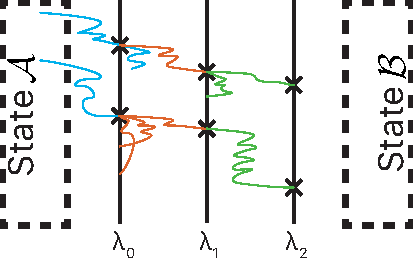
\includegraphics{{model_schematics/ffpilot_pilot_stage}.pdf}
    \end{center}
    \caption{Schematic example of a pilot stage from a FFPilot simulation, with total phase count $\Phase = 3$ and $\samplecountpilot = 2$. Trajectories from phases (blue) 0, (red) 1, and (green) 2 shown in different colors.}
    \label{fig:ffpilot_pilot_stage}
\end{figure}
\clearpage

\begin{figure}[h]
    \begin{center}
        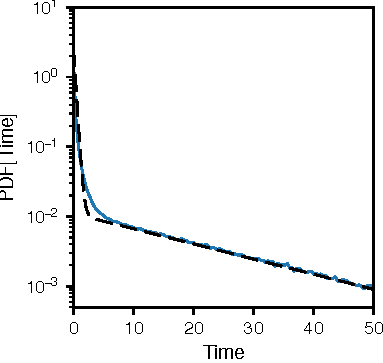
\includegraphics{{Figures/name_srg_-_ffpilot_phase_zero_dwell_time_dist_-_with_fit}.pdf}
    \end{center}
    \caption{Distribution of waiting times in between phase 0 forward flux events for $\SRGSLOW$, $10^6$ samples. Dashed line is a fit of a mixture of two exponential distributions.}
    \label{fig:name_srg_-_ffpilot_phase_zero_dwell_time_dist_-_with_fit}
\end{figure}
\clearpage

\begin{figure}[h]
    \begin{center}
        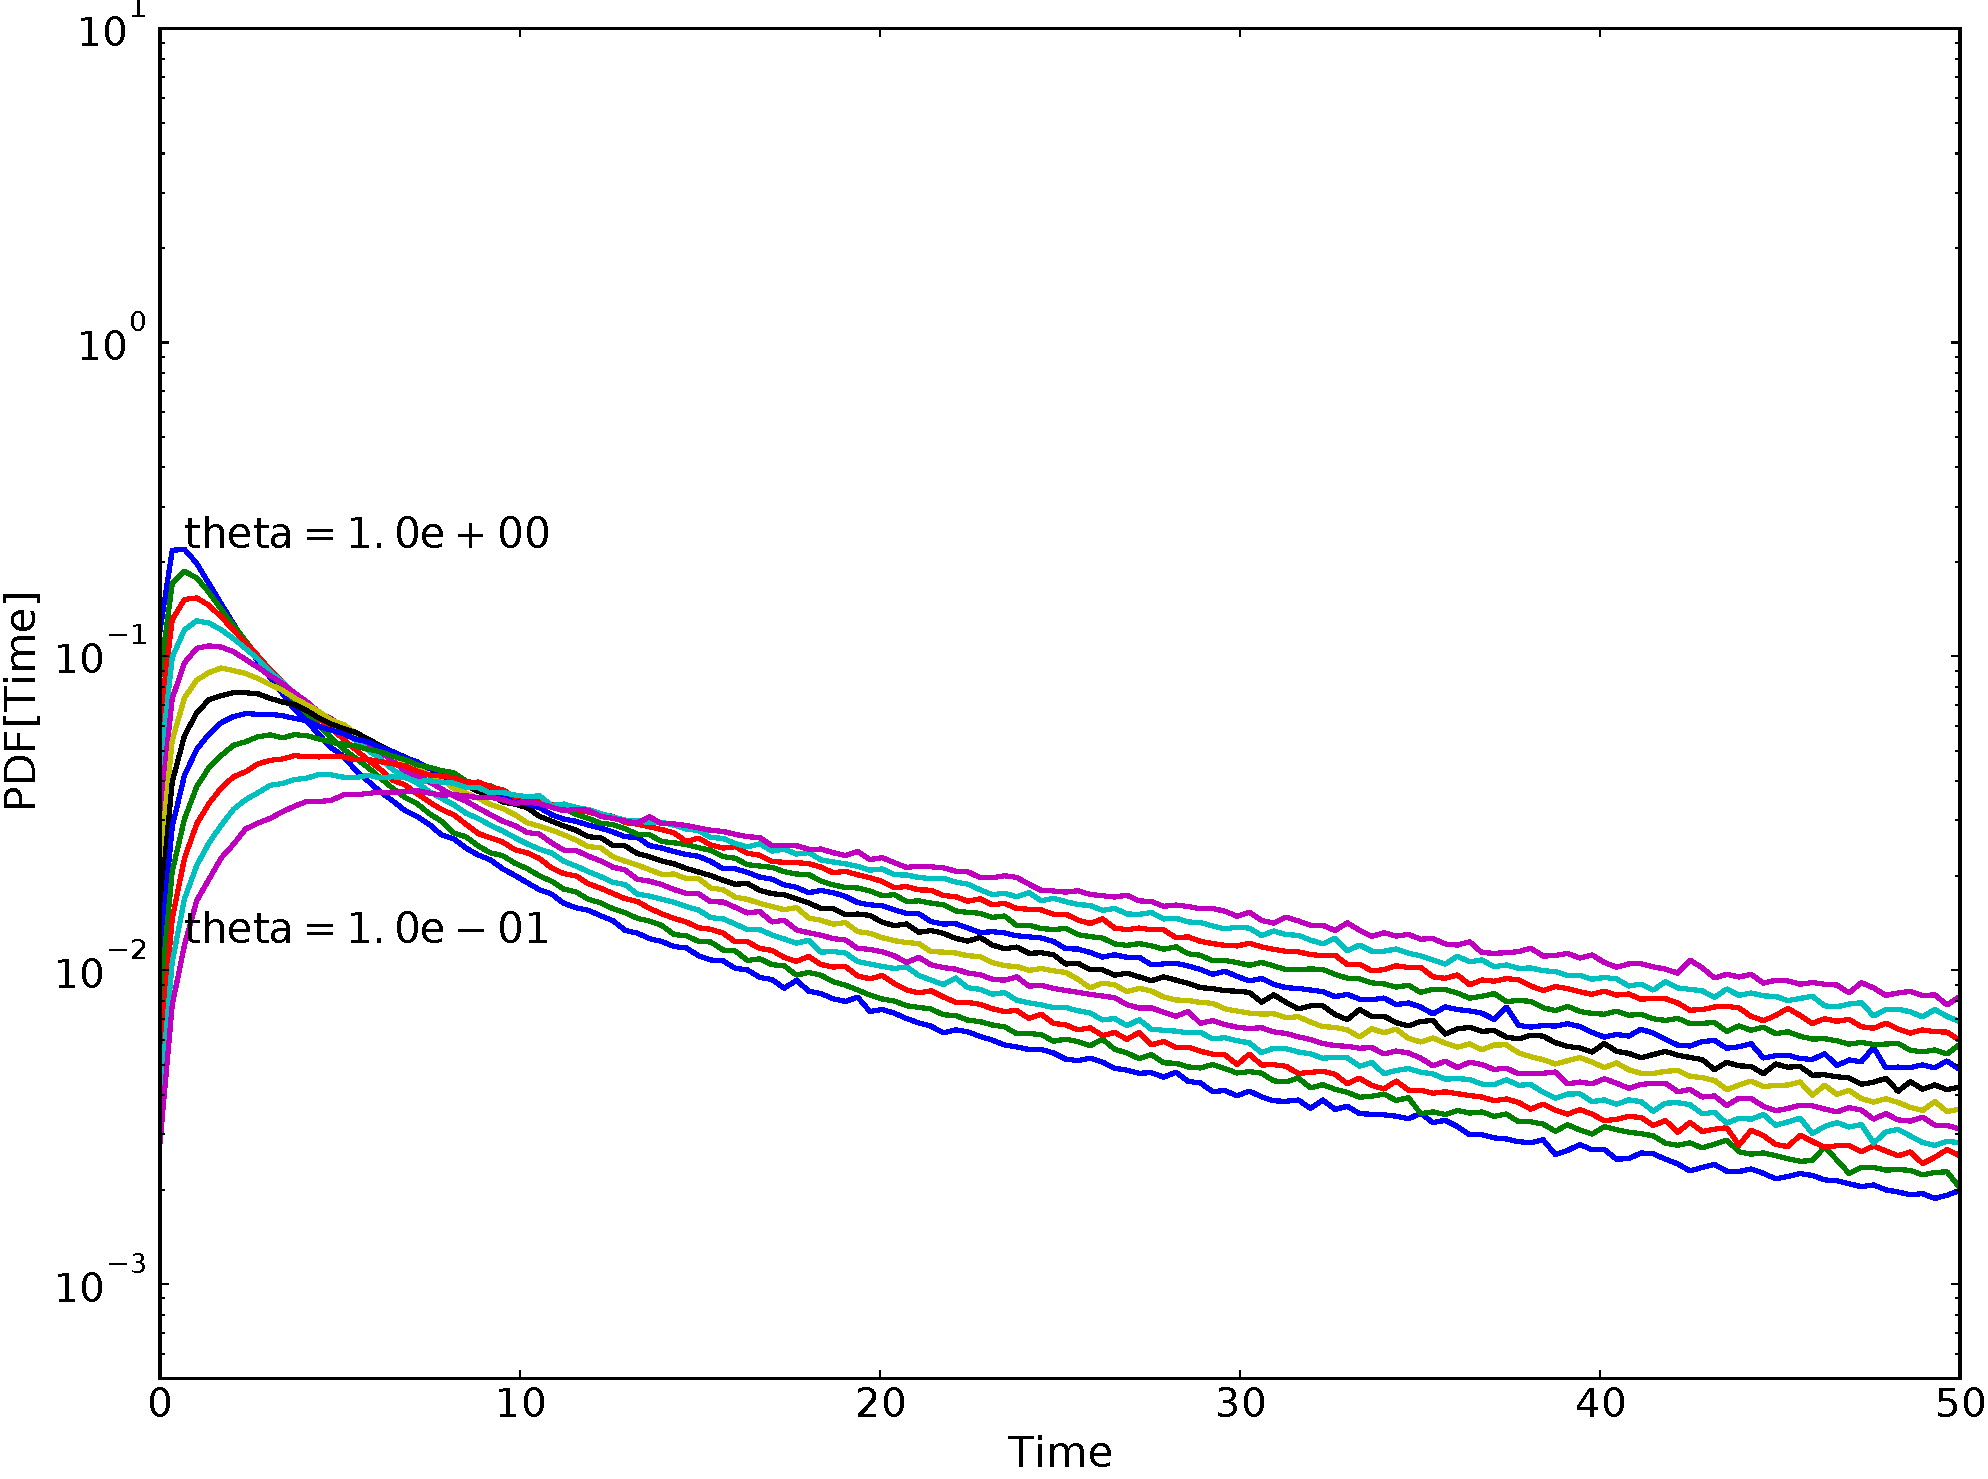
\includegraphics[width=\textwidth,height=\textheight,keepaspectratio]{{Figures/name_gts_-_ffpilot_phase_zero_dwell_time_dist_-_many_thetas_-_1e6_samples}.pdf}
    \end{center}
    \caption{Genetic Toggle Switch phase zero inter-event time distribution for values of $\theta$ in between $.1$ and $10$ (inclusive). $10^6$ samples in each distribution.}
    \label{fig:name_gts_-_ffpilot_phase_zero_dwell_time_dist_-_many_thetas_-_1e6_samples}
\end{figure}
\clearpage

\begin{figure}[h]
    \begin{center}
        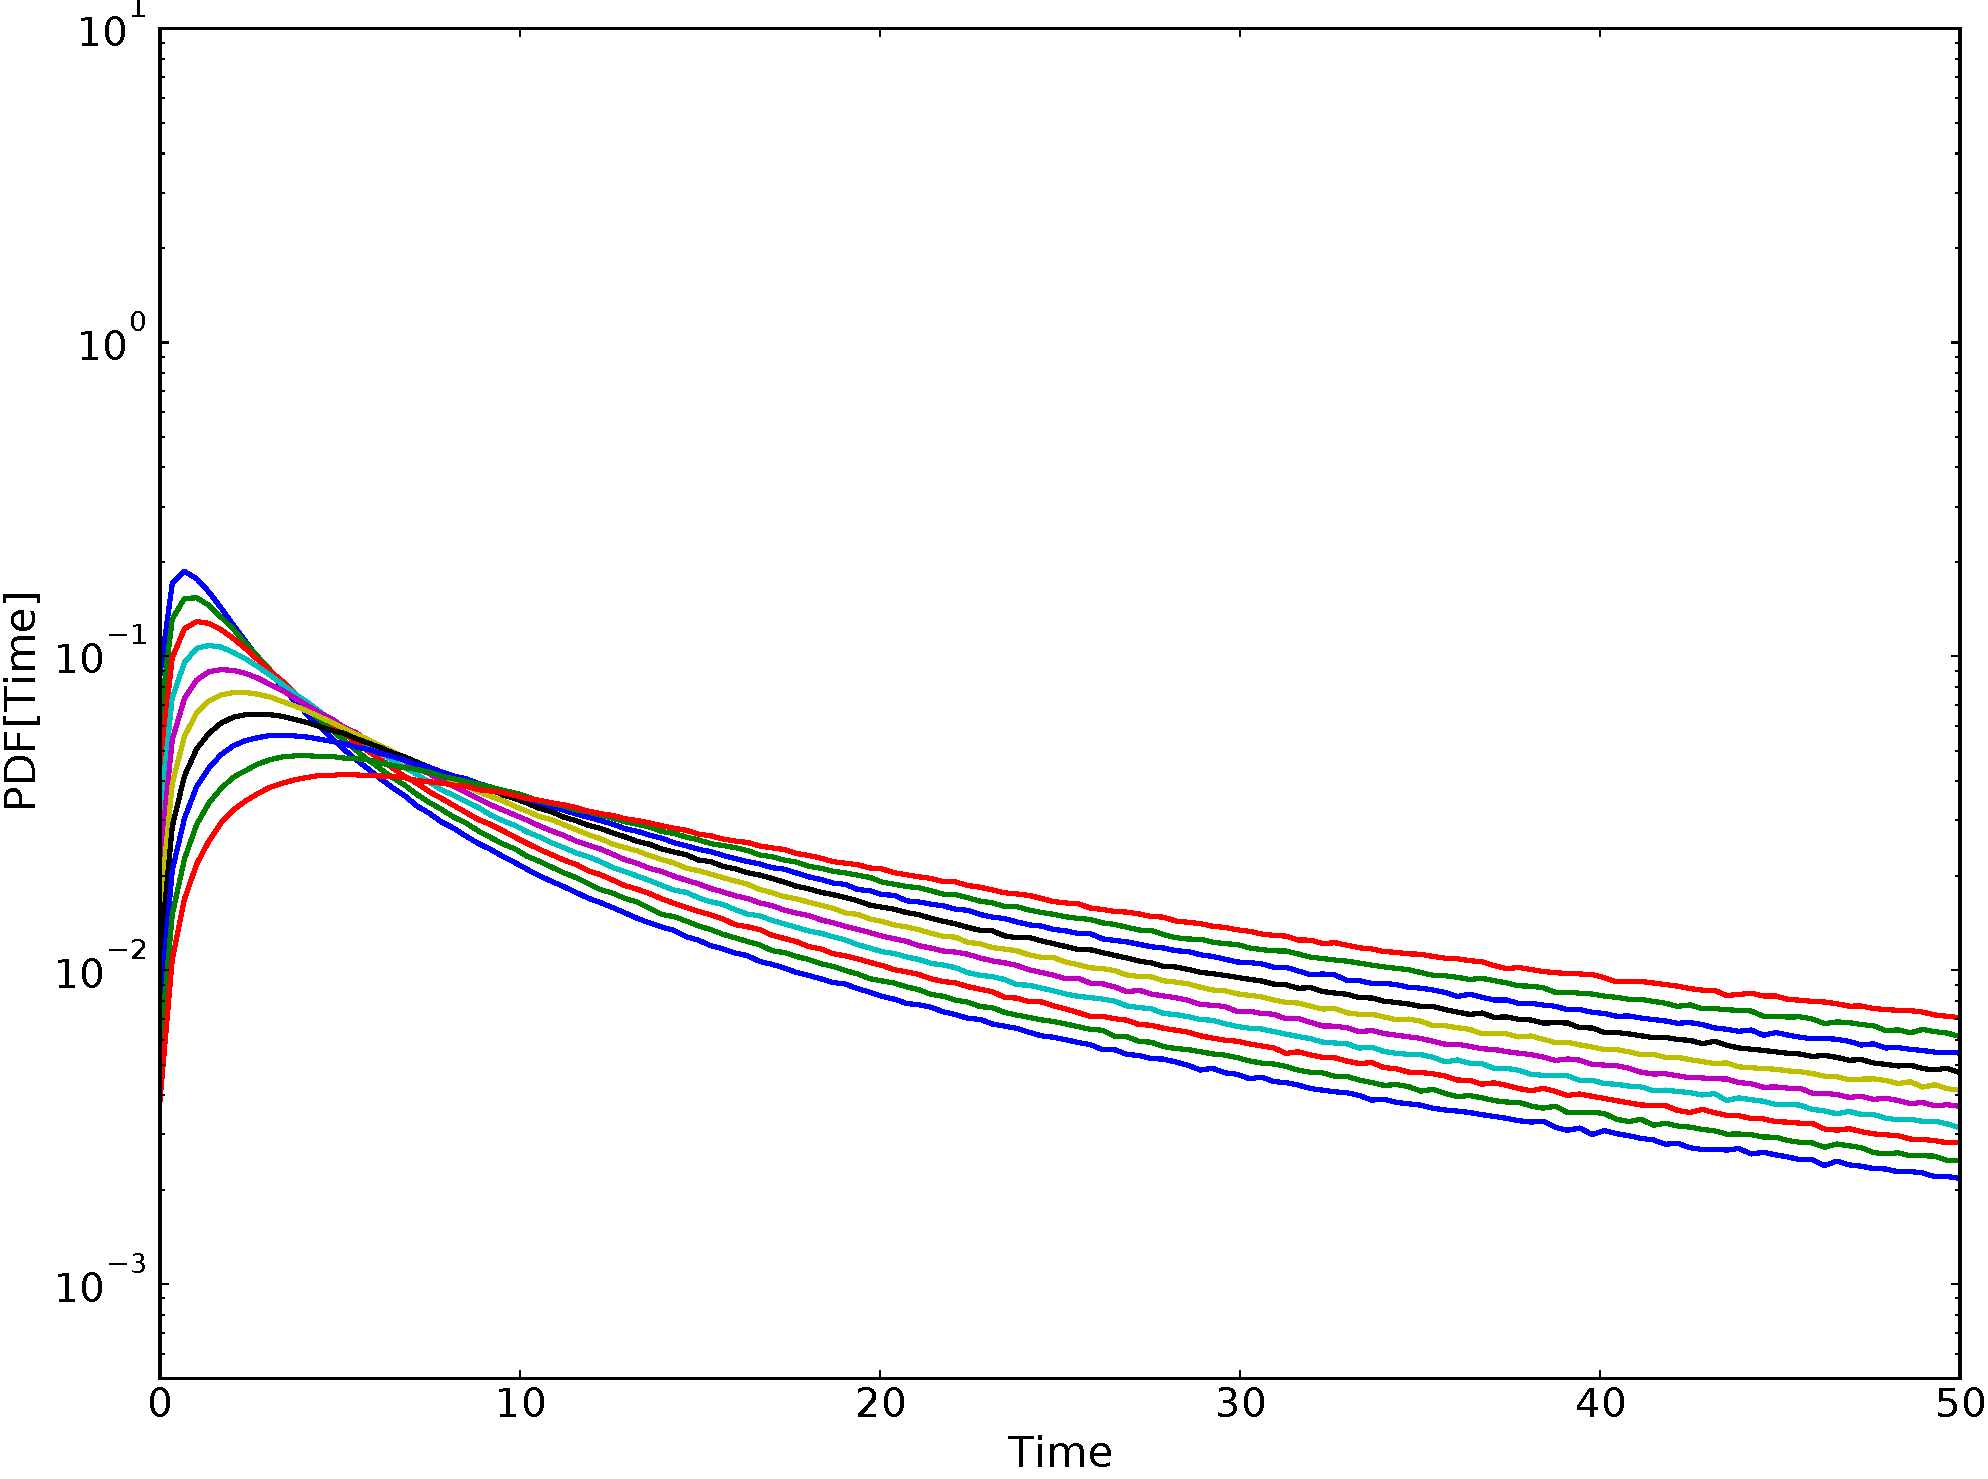
\includegraphics[width=\textwidth,height=\textheight,keepaspectratio]{{Figures/name_gts_-_ffpilot_phase_zero_dwell_time_dist_-_many_thetas_-_1e7_samples}.pdf}
    \end{center}
    \caption{Genetic Toggle Switch phase zero inter-event time distribution for values of $\theta$ in between $.1$ and $10$ (non-inclusive). $10^7$ samples in each distribution.}
    \label{fig:name_gts_-_ffpilot_phase_zero_dwell_time_dist_-_many_thetas_-_1e7_samples}
\end{figure}
\clearpage

%\begin{figure}[h]
%    \begin{center}
%        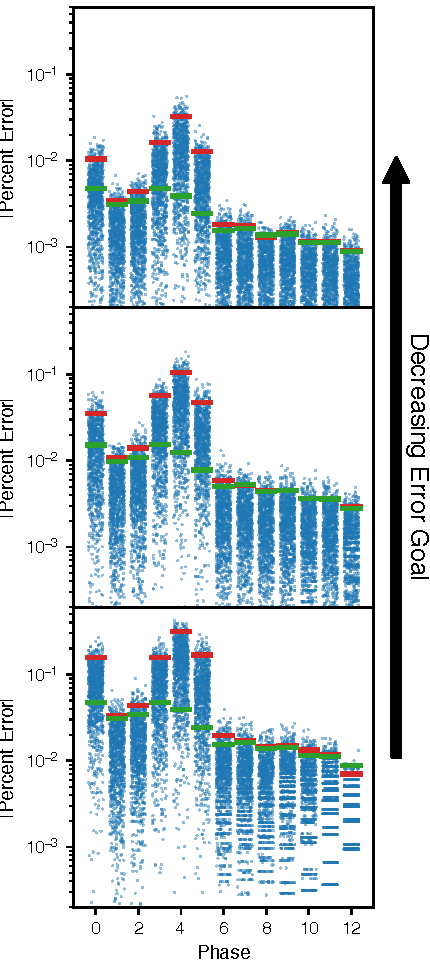
\includegraphics{{Figures/name_gts_-_phase_weight_percent_error_-_error_goal_all_-_pzs_multiplier__1.0e+00_-_theta_1.0e+01}.pdf}
%    \end{center}
%    \caption{Percent error of each phase weight from a set of FFPilot $\GTSSLOWEST$ simulations. The red line marks the 95th percentile of the error. The green line marks the location of the 95th error percentile as predicted by FFPilot at the end of the pilot stage. When the red line is at or below the green line, this means that FFPilot is controlling simulation error as expected.     The same phase zero sampling multiplier, 1X, was used for every simulation. Each subfigure represents results from simulations executed with a different error goal (from top to bottom, 10\%, 3.2\%, and 1\%).}
%    \label{fig:name_gts_-_phase_weight_percent_error_-_error_goal_all_-_pzs_multiplier__1.0e+00_-_theta_1.0e+01}
%\end{figure}
%\clearpage

\begin{figure}[h]
    \begin{center}
        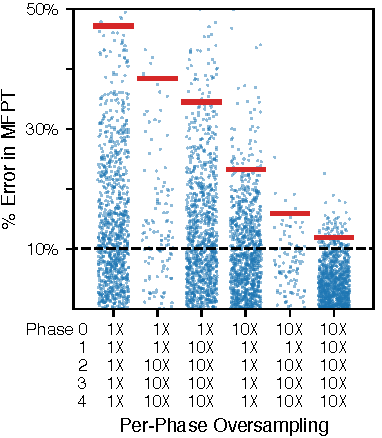
\includegraphics{{supplemental/figures/name_gts_-_stage_fpt_percent_error_-_landscape_fudge_pzs_multiplier_10_-_error_goal_1.0e-01_-_theta_1.0e+01}.pdf}
    \end{center}
    \caption{More results from simulations executed with various oversampling schemes. Aside from the use of 10X phase 0 oversampling instead of 20X, these simulations were equivalent to those presented in \figref{fig:name_gts_-_stage_fpt_percent_error_-_landscape_fudge_several_-_error_goal_1.0e-01_-_theta_1.0e+01} in the main paper. As can be seen in the righthand column, 10X oversampling in every phase from 0 to 4 is almost, but not quite, enough to eliminate landscape error. The extent of oversampling in each separate scheme is indicated beneath each column of results. 1X sampling implies that standard number of FFPilot trajectories were sampled in that phase. For purposes of comparison, results from simulations run with no oversampling are included in the first column, and results from simulations run with 10X phase 0, 10X phase 1-4 oversampling are also shown. All simulations were of $\GTSSLOW$ at an error goal of 10\%.}
    \label{fig:name_gts_-_stage_fpt_percent_error_-_landscape_fudge_pzs_multiplier_10_-_error_goal_1.0e-01_-_theta_1.0e+01}
\end{figure}
\clearpage

\begin{figure}[h]
    \begin{center}
        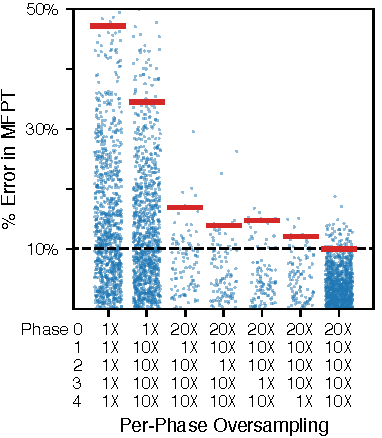
\includegraphics{{Figures/name_gts_-_stage_fpt_percent_error_-_landscape_fudge_skips_-_error_goal_1.0e-01_-_theta_1.0e+01}.pdf}
    \end{center}
    \caption{More results from simulations executed with various oversampling schemes. We wanted to investigate the effects of skipping oversampling in a single phase. Starting at the second column, results are shown from simulations in which we skipped oversampling in phase 0, then in the next column from simulations in which we skipped oversampling in phase 1, and so forth.     The extent of oversampling in each separate scheme is indicated beneath each column of results. 1X sampling implies that standard number of FFPilot trajectories were sampled in that phase. For purposes of comparison, results from simulations run with no oversampling are included in the first column, and results from simulations run with 20X phase 0, 10X phase 1-4 oversampling (which is enough to eliminate landscape error) are also shown. All simulations were of $\GTSSLOW$ at an error goal of 10\%.}
    \label{fig:name_gts_-_stage_fpt_percent_error_-_landscape_fudge_skips_-_error_goal_1.0e-01_-_theta_1.0e+01}
\end{figure}
\clearpage

\begin{figure}[h]
    \begin{center}
        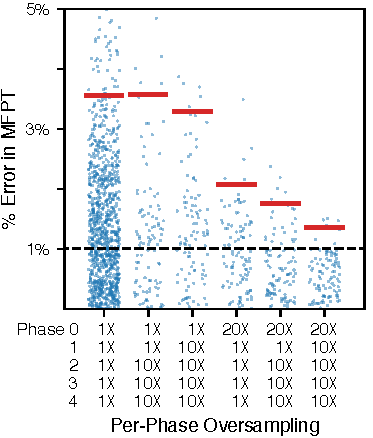
\includegraphics{{supplemental/figures/name_gts_-_stage_fpt_percent_error_-_landscape_fudge_several_-_referenceMFPT_highacc_-_error_goal_1.0e-02_-_theta_1.0e+01}.pdf}
    \end{center}
    \caption{$\mfpttrue$ percent errors from a large set of simulations executed with various oversampling schemes. The simulations are similar to those presented in \figref{fig:name_gts_-_stage_fpt_percent_error_-_landscape_fudge_several_-_error_goal_1.0e-01_-_theta_1.0e+01} from the main paper, except that all simulations were of $\GTSSLOW$ at an error goal of 1\% instead of 10\%. All $\mfpttrue$ percent errors are calculated relative to the $\mfpttrue$ value estimated by a high accuracy DS simulation (.62\% error goal).}
    \label{fig:name_gts_-_stage_fpt_percent_error_-_landscape_fudge_several_-_referenceMFPT_highacc_-_error_goal_1.0e-02_-_theta_1.0e+01}
\end{figure}
\clearpage

\begin{figure}[h]
    \begin{center}
        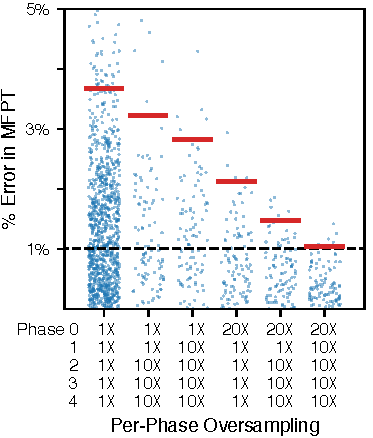
\includegraphics{{supplemental/figures/name_gts_-_stage_fpt_percent_error_-_landscape_fudge_several_-_referenceMFPT_highaccFFPilot_-_error_goal_1.0e-02_-_theta_1.0e+01}.pdf}
    \end{center}
    \caption{$\mfpttrue$ percent errors from a large set of simulations executed with various oversampling schemes. The simulations are similar to those presented in \figref{fig:name_gts_-_stage_fpt_percent_error_-_landscape_fudge_several_-_error_goal_1.0e-01_-_theta_1.0e+01} from the main paper, except that all simulations were of $\GTSSLOW$ at an error goal of 1\% instead of 10\%. All $\mfpttrue$ percent errors are calculated relative to the $\mfpttrue$ value estimated by a high accuracy FFPilot simulation (.1\% error goal).}
    \label{fig:name_gts_-_stage_fpt_percent_error_-_landscape_fudge_several_-_referenceMFPT_highaccFFPilot_-_error_goal_1.0e-02_-_theta_1.0e+01}
\end{figure}
\clearpage

\begin{comment}
\begin{figure}[h]
    \begin{center}
        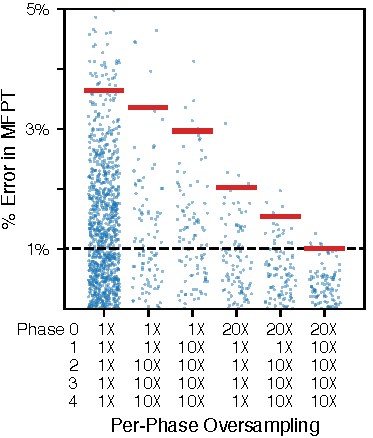
\includegraphics{{supplemental/figures/name_gts_-_stage_fpt_percent_error_-_landscape_fudge_several_-_referenceMFPT_mean_-_error_goal_1.0e-02_-_theta_1.0e+01}.pdf}
    \end{center}
    \caption{$\mfpttrue$ percent errors from a large set of simulations executed with various oversampling schemes. The simulations are similar to those presented in \figref{fig:name_gts_-_stage_fpt_percent_error_-_landscape_fudge_several_-_error_goal_1.0e-01_-_theta_1.0e+01} from the main paper, except that all simulations were of $\GTSSLOW$ at an error goal of 1\% instead of 10\%. In this version of the figure, all $\mfpttrue$ percent errors are calculated relative to the mean $\mfpttrue$ value estimated by all of the simulations within that particular oversampling condition.}
    \label{fig:name_gts_-_stage_fpt_percent_error_-_landscape_fudge_several_-_referenceMFPT_mean_-_error_goal_1.0e-02_-_theta_1.0e+01}
\end{figure}
\clearpage    
\end{comment}

\begin{figure}[h]
    \begin{center}
        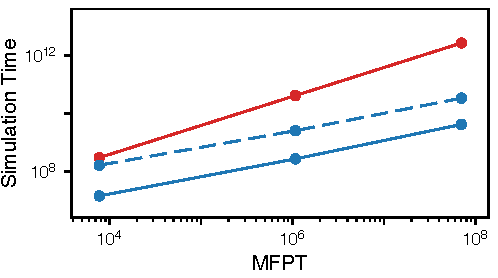
\includegraphics{{Figures/name_theta_-_speedup_plot_-_simtime_vs_mfpt_-_error_goal_1.0e-02}.pdf}
    \end{center}
    \caption{Simulation time vs \abr{MFPT} for several \abr{SRG} models. The simulation time for both \abr{DS} (red lines) and \abr{FFPilot} (blue lines) are shown.} 
    \label{fig:name_h_-_speedup_plot_-_simtime_vs_mfpt_-_error_goal_1.0e-02}
\end{figure}
\clearpage

\begin{figure}[h]
    \begin{center}
        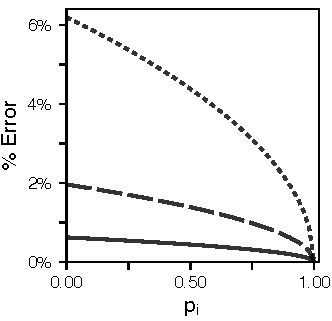
\includegraphics{{Figures/blind_optimization_-_percent_error_vs_pi_-_several_success_counts}.pdf}
    \end{center}
    \caption{Maximum error (with respect to a single phase weight, 95\% confidence) vs phase weight for a phase $\phasegz$ when using the blind optimization method from the \abr{FFPilot} pilot stage. Each of the lines shows the error for a different fixed value of the successful trajectory count, $\successcount = \samplecountpilot$. (solid line) $\samplecountpilot = 10^5$, (dashed line) $\samplecountpilot = 10^4$, (dotted line) $\samplecountpilot = 10^3$.}
    \label{fig:blind_optimization_-_percent_error_vs_pi_-_several_success_counts}
\end{figure}
\clearpage

\begin{figure}[h]
    \begin{center}
        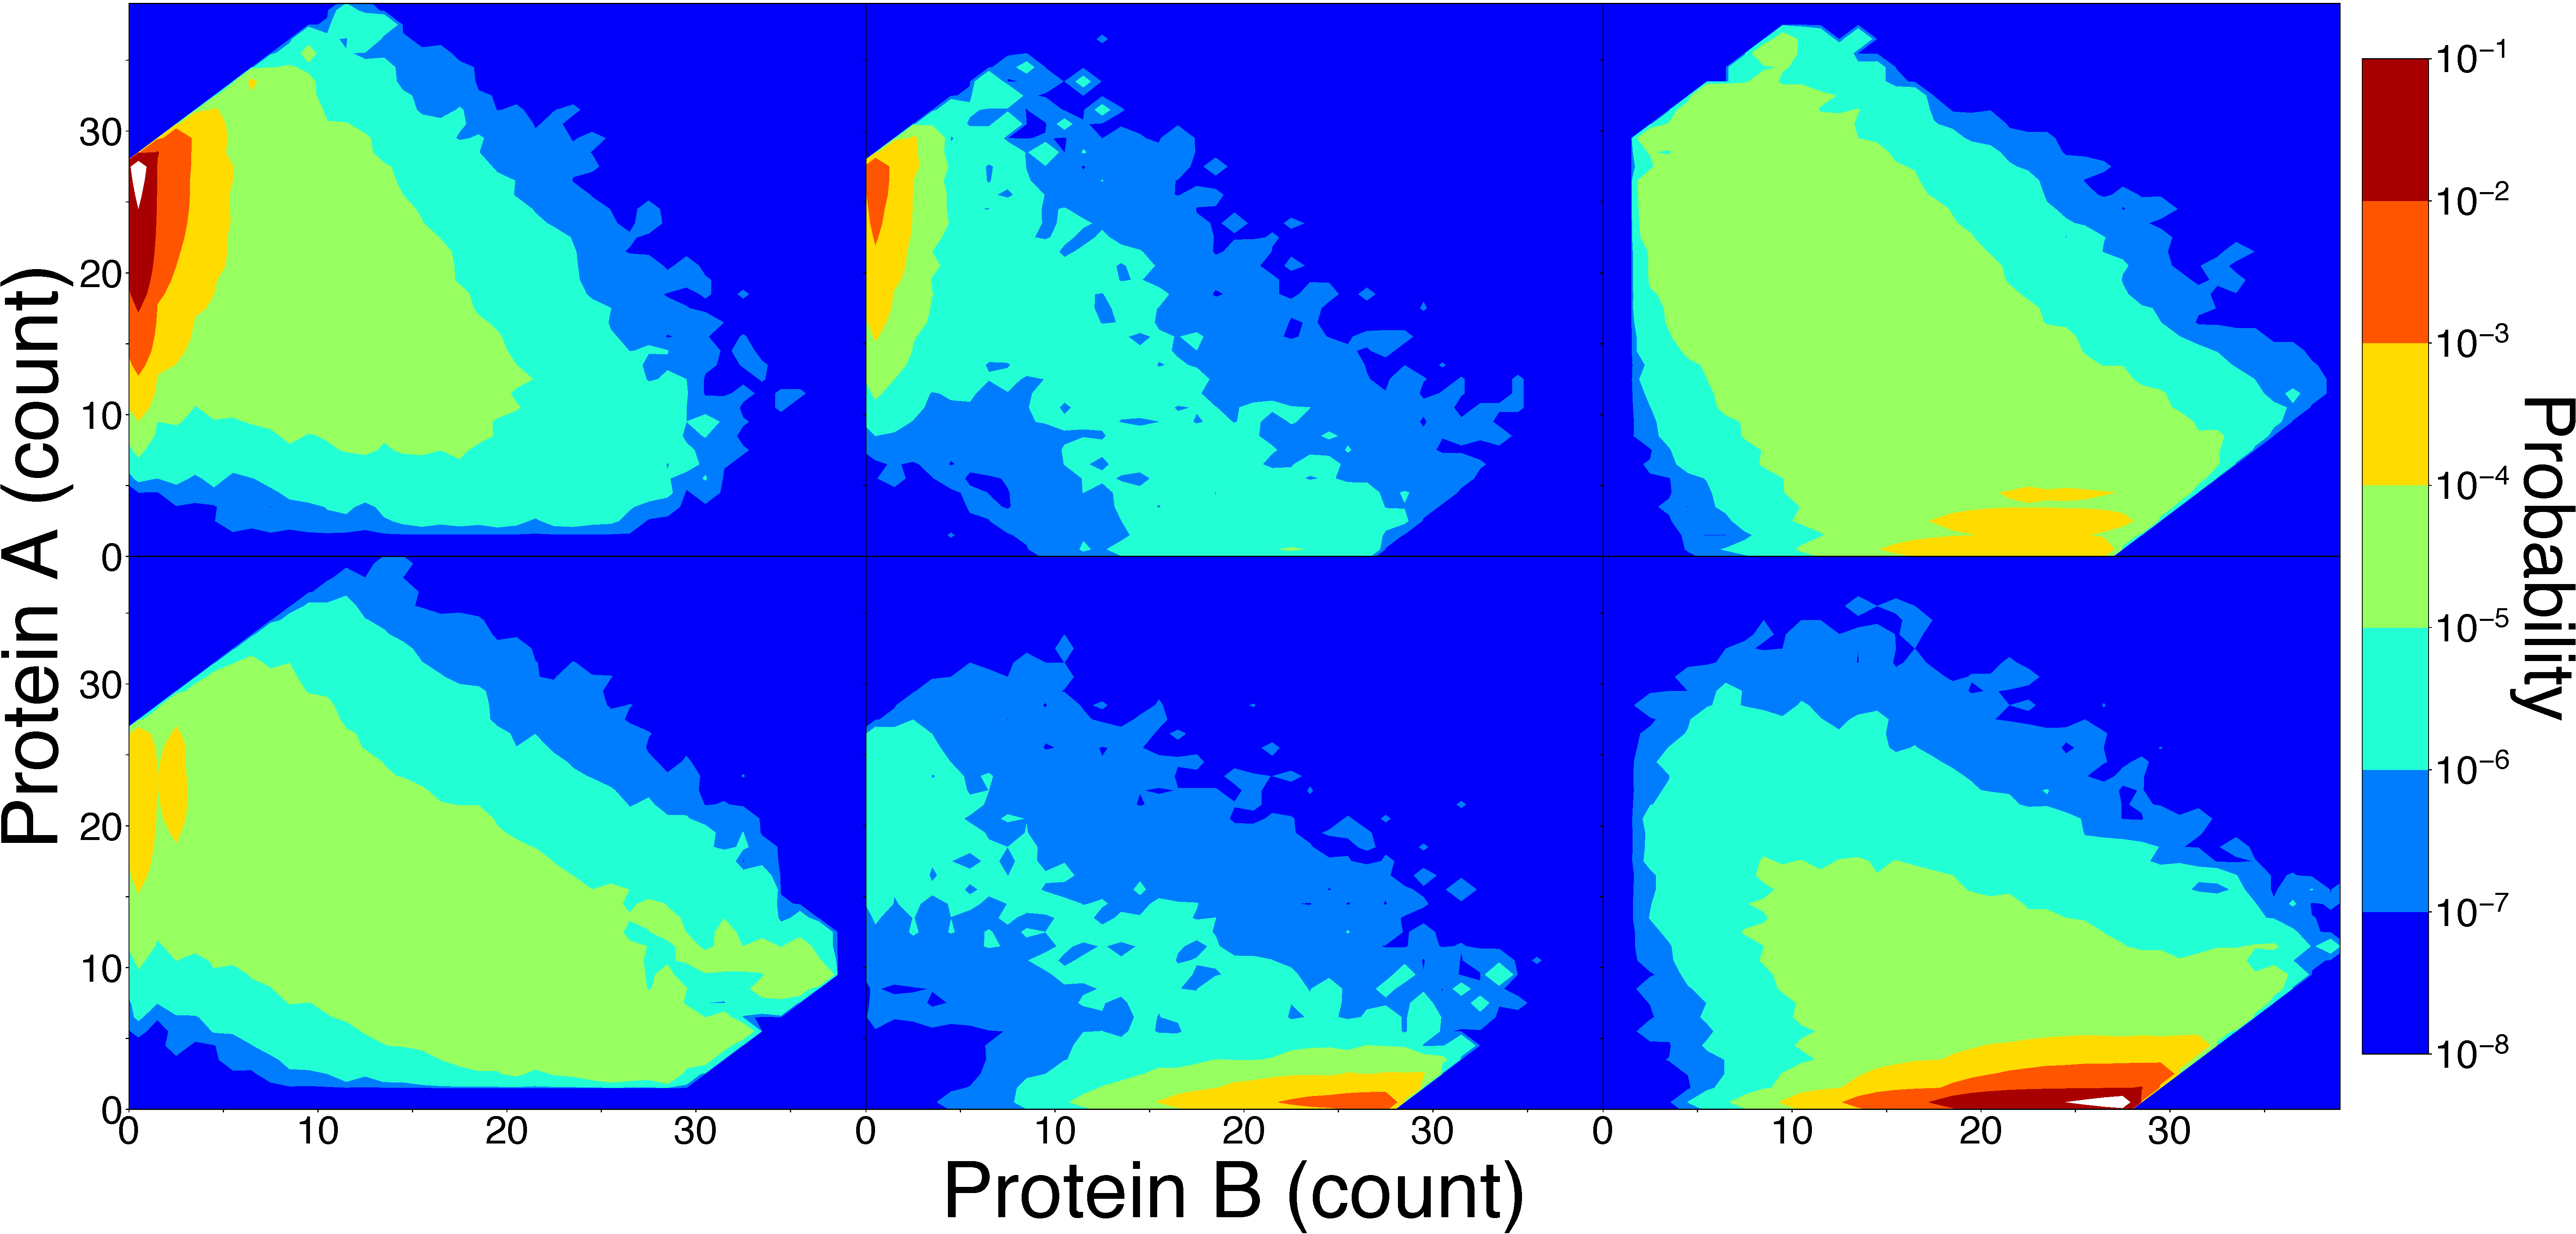
\includegraphics[width=\textwidth,height=\textheight,keepaspectratio]{{Figures/name_gts_-_landscape_operator_slices_-_plot_contour}.pdf}
    \end{center}
    \caption{The state landscape of $\GTSSLOW$, sliced by operator occupancy. The lefthand column shows the slice of the landscape in which an A dimer is bound to the operator DNA, the middle column shows the slice in which the operator is unbound, and the righthand column shows the slice in which the operator is bound to a B dimer. The top row is from a simulation of $\GTSSLOW$ in which it switched $\atob$, and the bottom row is from a simulation in which it switch $btoa$. Complex, high dimensional, and reasonably accurate landscapes can be produced in a straightforward fashion from relatively low cost \abr{FFPilot} simulations. The 3 landscapes in each row represent the output of a single \abr{FFPilot} simulation run to a 10\% error goal, which ran to completion on a laptop in ~5 minutes. The landscapes were analyzed and plotted using LMA, an analysis package written in Python and designed to work alongside the Lattice Microbes simulation suite.}
    \label{fig:name_gts_-_landscape_operator_slices_-_plot_contour}
\end{figure}
\clearpage

%\end{document}

